\documentclass{article}
\usepackage[utf8]{inputenc}
\usepackage{amsmath}
\usepackage{graphicx}
\usepackage{BeginnerStyleFile}
\graphicspath{ {images/} }

\title{Reading Summary 4.2}
\author{Evan Hughes}
\date{March 2023}

\begin{document}
\maketitle
\section*{4.2 Divisibility in $F[x]$}
All the results of Section 1.2 on divisibility and greatest common divisors in $\mathbb{Z}$ now
carry over, with only minor modifications, to the ring of polynomials over a field.
Throughout this section, $F$ always denotes a field. 

\subsection*{Definition} Let $F$ be a field and $a(x), b(x) \in F[x]$. We say that $b(x)$ divides $a(x)$, and write $b(x) \mid a(x)$, if $a(x) = b(x)h(x)$ for some $h(x) \in F[x]$.

\subsection*{Example (from the book)} $(2x+1)\mid(6x^2-x-2)$ in $\mathbb{Q}[x]$ because $6x^2-x-2 = (2x+1)(3x-2)$.

\subsection*{Theorem 4.7}
Let $F$ be a field and $a(x), b(x) \in F[x]$ with $b(x)$ nonzero.
\begin{enumerate}
    \item If $b(x)$ divides $a(x)$, then $cb(x)$ divides $a(x)$ for any nonzero $c \in F$.
    \item Every divisor of $a(x)$ has degree less than or equal to deg $a(x)$.
\end{enumerate}

\subsection*{Proof of Theorem 4.7}
\begin{enumerate}
    \item If $b(x)$ divides $a(x)$, then $a(x) = b(x)h(x)$ for some $h(x) \in F[x]$. Hence
    \begin{equation}
        a(x) = 1_F \cdot b(x)h(x) = c^-1b(x)h(x) = cb(x)[c^-1h(x)]
    \end{equation}

    Therefore, $cb(x)\mid a(x)$
    \item Suppose $b(x)\mid a(x)$, say $a(x) = b(x)h(x)$. By Theorem 4.2, deg $a(x) = $ deg $b(x) + $ deg $h(x)$.
    Since degrees are nonnegative, we must have $0 \leq$ deg $b(x) \leq$ deg $a(x)$.
\end{enumerate}


\subsection*{Definition}
Let $F$ be a field and $a(x), b(x) \in F[x]$, not both zero. The greatest common divisor(gcd) of
$a(x)$ and $b(x)$ is the monic polynomial of highest degree that divides both $a(x)$ and $b(x)$.

In other words, $d(x)$ is the gcd of $a(x)$ and $b(x)$ if and only if $d(x)$ is a monic and
\begin{enumerate}
    \item $d(x)$ divides $a(x)$ and $d(x)$ divides $b(x)$
    \item If $c(x)$ divides $a(x)$ and $c(x)$ divides $b(x)$, then deg $c(x) \leq$ deg $d(x)$
\end{enumerate}

Polynomials $a(x)$ and $b(x)$ have at least one monic common divisor(namely $1_p$), Since
the degree of a common divisor of $a(x)$ and $b(x)$ cannot exceed either deg $a(x)$ or deg $b(x)$
by Theorem 4.7, there must be at least one monic common divisor of highest degree. In
Theorem 4.8 below we shall show that there is only one monic common divisor of highest
degree, thus justifying the definition's reference to the greatest common divisor.

\subsection*{Example}

You can verify factorization in $\mathbb{Q}[x]$ by using the gcd of two polynomials. For example, $(x^2-1)(x^2+1) = x^4-1$.
and $(2x+1)(x-2)x = 2x^3-3x^2-2x$. in this example $2x+1$ is the common divisor of the highest degree.

\subsection*{Theorem 4.8}
Let $F$ be a field and $a(x), b(x) \in F[x]$, not both zero. Then there is a unique greatest common divisor
$d(x)$ of $a(x)$ and $b(x)$. Futhermore, there are polynomials $u(x)$ and $v(x)$ such that
$d(x) = a(x)u(x) + b(x)v(x)$.

\subsection*{Proof of Theorem 4.8}

Step 1: Find a monic polynomial of smallest degree in $S$.

Proof of Step 1: $S$ contains nonzero polynomials. So the set of all
degrees of polynomials in $S$ is a nonempty set of nonnegative integers.
which has a smallest element by the Well-Ordering Axiom. Hence, there
is a polynomial $w(x)$ of smallest degree in $S$. If $d$ is the leading coefficient of $w(x)$, then $t(x) = d^-1 w(x)$ 
is a monic polynomial of smallest
degree in $S$. By the definition of $S$,
\begin{center}
    $t(x) = a(x)u(x) + b(x)v(x)$ for some $u(x), v(x) \in F[x]$
\end{center}

Step 2: Prove that $t(x)$ is the gcd of $a(x)$ and $b(x)$.

Proof of Step 2: We must prove that $t$ satisfies the two conditions in the definition of gcd:
\begin{enumerate}
    \item $t(x)$ divides $a(x)$ and $t(x)$ divides $b(x)$
    \item If $c(x)$ divides $a(x)$ and $c(x)$ divides $b(x)$, then deg $c(x) \leq$ deg $t(x)$
\end{enumerate}

Proof of 1: Same as proof of Theorem 1.2, but with coefficient rings.

Proof of 2: Same as proof of Theorem 1.2, but with coefficient rings.

Step 3: Prove that $t(x)$ is unique.
Proof of Step 3: Suppose that $d(x)$ is any gcd of $a(x)$ and $b(x)$. To prove
uniqueness, we must show that $d(x) = t(x)$. Since $d(x)$ is a common divisor,
we have $a(x) = d(x)f(x)$ and $b(x) = a(x)g(x)$ for some $f(x), g(x) \in F[x]$.

Therefor,

$t(x) = a(x)u(x) + b(x)v(x) = d(x)f(x)u(x) + d(x)g(x)v(x) = d(x)[f(x)u(x) + g(x)v(x)]$

By Theorem 4.2, deg $t(x) = $ deg $d(x) + $ deg $[f(x)u(x) + g(x)v(x)]$.

Since they are gcds, $t(x)$ and $d(x)$ have the same degree. Hence, $[f(x)u(x) + g(x)v(x)] = 0 $,
so that $f(x)u(x) + g(x)v(x) = c$ for some constant $c \in F$. Therefore,
$t(x) = d(x)c$. Since both $t(x)$ and $d(x)$ are monic, the leading coefficient on the left side is $1_F$ and the leading
coefficient on the right side is $c$. So we must have $c = 1_F$. Therefore, $d(x)
= t(x) = a(x)u(x) + b(x)v(x)$ is the unique gcd of $a(x)$ and $b(x)$.

\subsection*{Corollary 4.9}
Let $F$ be a field and $a(x), b(x) \in F[x]$, not both zero. A monic polynomial
$d(x) \in F[x]$ is a gcd of $a(x)$ and $b(x)$ if and only if $d(x)$ satisfies these conditions.

\begin{itemize}
    \item $d(x)$ divides $a(x)$ and $d(x)$ divides $b(x)$
    \item if $c(x)$ divides $a(x)$ and $c(x)$ divides $b(x)$, then $c(x)$ divides $d(x)$
\end{itemize}

\subsection*{Proof of Corollary 4.9}
Adapt the proof of Corollary 1.3 to $F[x]$.

\subsection*{Theorem 4.10}
Let $F$ be a field and $a(x), b(x), c(x) \in F[x]$. If $a(x) \mid b(x)c(x)$ and $a(x)$ and $b(x)$ are relatively prime, then $a(x) \mid c(x)$.


\begin{figure}
    \centering
    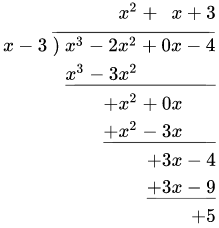
\includegraphics[width=0.3\textwidth]{polynomialdivision.png}
    \caption{Polynomial Division}
    \label{fig:division_algorithm}
\end{figure}
\end{document}